\documentclass[answers]{exam}

\usepackage{graphicx}
\usepackage{float}
\usepackage{amsmath}
\usepackage{subcaption}
\usepackage{framed}
\usepackage{amsthm}
\usepackage{amsmath}
\usepackage{amsfonts}
\usepackage{algorithmicx}
\usepackage{algpseudocode}
\usepackage{mathtools}
\usepackage{tikz}
\newcommand\numberthis{\addtocounter{equation}{1}\tag{\theequation}}
\newtheorem{lemma}{Lemma}
\newtheorem{claim}{Claim}
\usepackage{etoolbox}
\AtBeginEnvironment{solution}{\setcounter{claim}{0}}

\usetikzlibrary{fit}
\newcommand\addvmargin[1]{
  \node[fit=(current bounding box),inner ysep=#1,inner xsep=0]{};
}

\DeclareMathOperator*{\argmax}{arg\,max}

\newcommand{\nl}{\vspace{0.2cm}\\}
\newcommand{\nln}{\vspace{0.2cm}}
 
% First we setup the header and footer
\pagestyle{headandfoot}
\runningheadrule
\runningfootrule
\header{COL351: Analysis and Design of Algorithms (CSE, IITD, Semester-I-2020-21)}{}{Homework-4}
\footer{}{\thepage  \, of \numpages}{}
 
% We want the points for each question displayed on the left
%\pointname{points}
%\pointsinmargin
 
% Automatically total the points - make sure to compile TWICE
\addpoints
 
\begin{document}


\begin{center} 
\fbox{\parbox{5.5in}{
%\vspace{-0.1in}
\begin{itemize}
\item \small{The instructions are the same as in Homework-0, 1, 2.}
\end{itemize}
%\vspace{-0.1in}
}}
\end{center}

%\vspace{0.1in}


%\vspace{0.1in}
% Some general text together with number of questions and total points possible
There are \numquestions\, questions for a total of \numpoints\, points.
%\vspace{0.1in}
\hrule
 %\vspace{0.2in}
\begin{questions}
 
% First question, worth 3 points
\question ({\it Please note that this question will be counted towards Homework-3.})

Consider two binary strings $x = x_1, ... x_n$ and $y = y_1, ..., y_m$. 
An interleaving of $x$ and $y$ is a strings $z = z_1, ..., z_{n+m}$ so that the bit positions of $z$ can be partitioned into two disjoint sets $X$ and $Y$ , so that looking only at the positions in $X$, the sub-sequence of $z$ produced is $x$ and looking only at the positions of $Y$ , the sub-sequence is $y$. 
For example, if $x = 1010$ and $y = 0011$, then $z = 10001101$ is an interleaving because the odd positions of $z$ form $x$, and the even positions form $y$. 
The problem is: given $x,y$ and $z$, determine whether $z$ is an interleaving of $x$ and $y$.

Here is a simple back-tracking recursive algorithm for this problem, based on the two cases:  If $z$ is an interleaving, either the first character in $z$ is either copied from $x$ or from $y$. 


\begin{framed}
{\tt BTInter($x_1, ..., x_n$ ; $y_1, ..., y_m$; $z_1, ..., z_{n+m}$)}:\\
\hspace*{0.1in} - IF $n=0$ THEN IF  $y_1, ..., y_m$ = $z_1, ..., z_m$ THEN return True ELSE return False\\
\hspace*{0.1in} - IF $m=0$ THEN IF $x_1, ..., x_n$ = $z_1, ..., z_n$ THEN return True ELSE return False\\
\hspace*{0.1in} - IF $x_1$ = $z_1$ AND {\tt BTInter($x_2, ..., x_n$, $y_1, ..., y_m$; $z_2, ..., z_{n+m}$}) return True\\
\hspace*{0.1in} - If $y_1$ = $z_1$.  AND {\tt BTInter($x_1, ..., x_n$, $y_2, ..., y_m$; $z_2, ..., z_{n+m}$}) return True\\
\hspace*{0.1in} - Return False 
\end{framed}

Answer the parts below:
\begin{parts}
\part[3] Show the tree of recursions the above algorithm would make on the above example.
\begin{solution}
\begin{figure}[H]
    \centering
    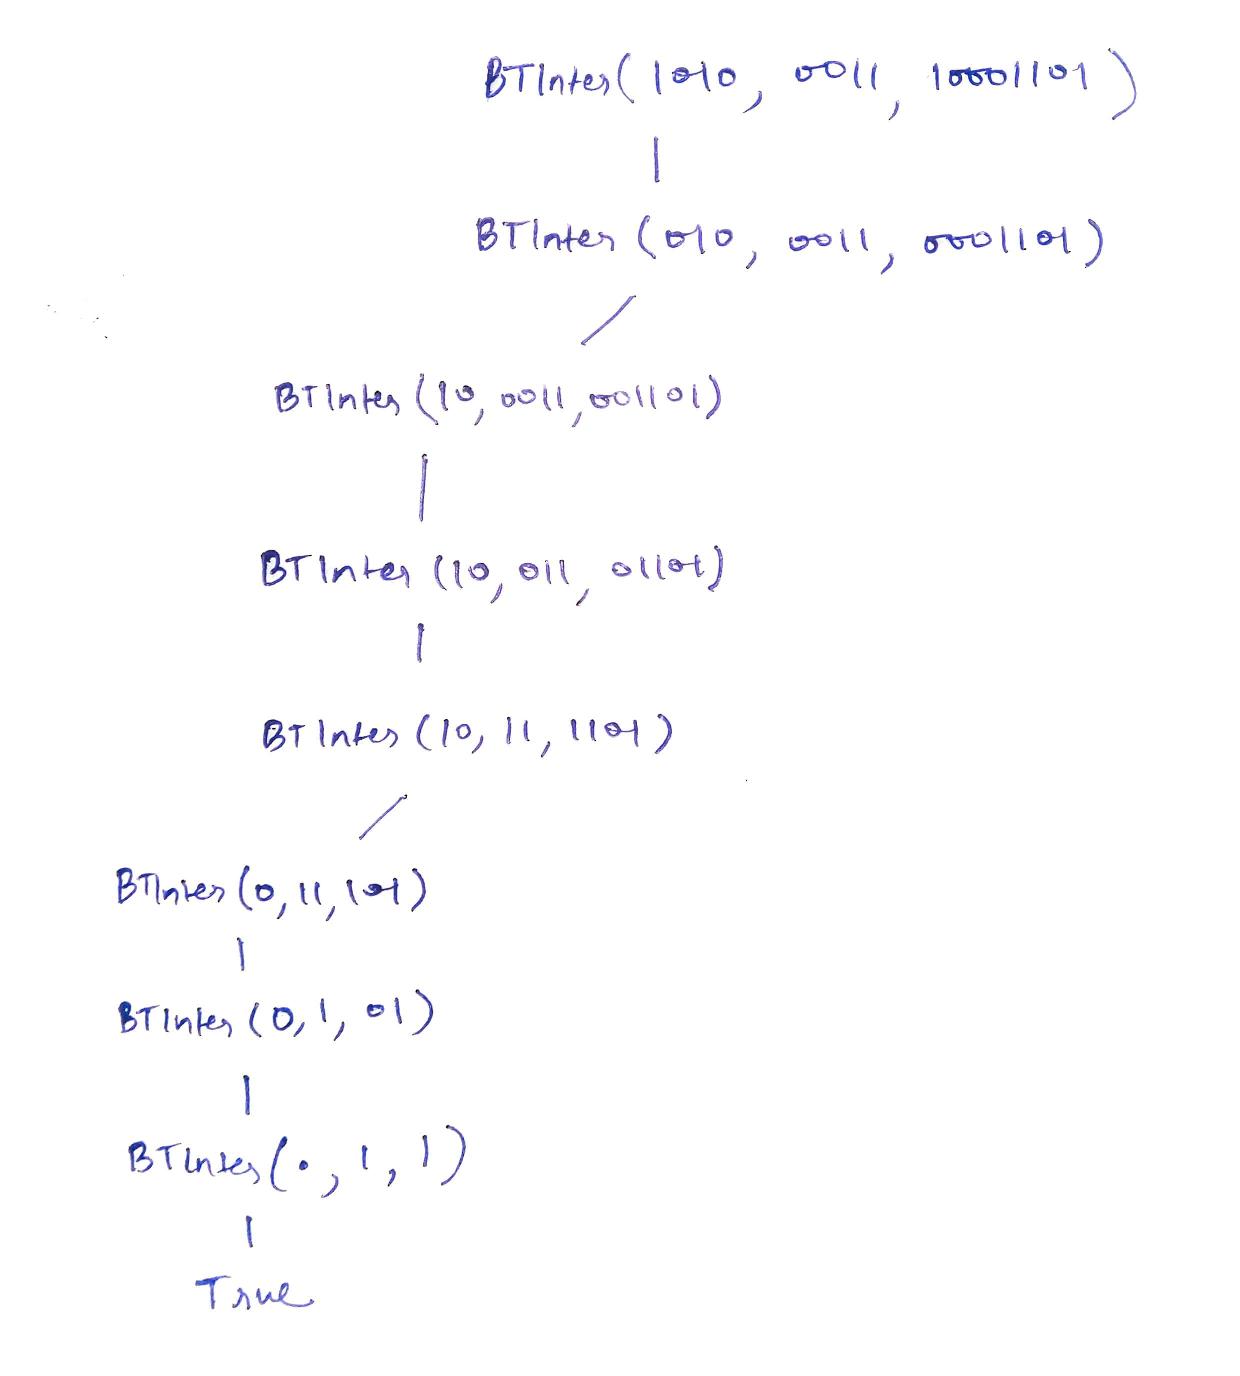
\includegraphics[width=0.5\textwidth]{embed/backtracking.pdf}
\end{figure}
\end{solution}

\part[3] Give an upper bound on the total number of recursive calls this algorithm might make in terms of $n$ and $m$.
\begin{solution}
In the worst case the algorithm will branch on both the possibilities, that is, $x_1 = y_1 = z_1$. In the base case when $n=0$ or $m=0$ the algorithm does string matching only and no recursive calls. In the other case, in the worst case, we make 2 recursive calls which make some recursive calls of their own. So let $T(n,m)$ denote the recursive calls made (not the time taken). Then, we can write the recurrence relation in terms of $n, m$ as 
\begin{align*}
    T(n, m) &\leq 
    \begin{cases}
        0 & n=0 \\
        0 & m=0 \\
        T(n-1, m) + T(n, m-1) + 2 & \text{otherwise}
    \end{cases}
\end{align*}
% \begin{claim}
% For all valid $n, m$, we have $T(n, m) \leq 2\binom{m+n}{m} - 2$.
% \end{claim}
% \begin{proof}
% We will prove the claim by induction on $m+n$ (breaking ties with $\min(n, m)$). First in the base case we will show how it is true when $n=0$ or $m=0$ then we complete the proof using the inductive argument. Note that here we will apply induction as follows, first in the base case we verify for $T(n,0)$ and $T(0,m)$ for all $n,m > 0$.

% \paragraph{Base Case} When $n=0, m>0$ or $m=0, n>0$. The algorithm will make no recursive calls. Clearly, $2\binom{m}{m} - 2 = 0$ and $2\binom{n}{0} - 2 = 0$ for $m,n > 0$ so the base case holds.
% \paragraph{Inductive Case} Suppose we have shown the claim for all values $\leq m+n-1$ for some $m, n > 0$. We will now show that this implies that the claim holds for $m+n$ as well.
% \begin{align*}
%     T(n,m) &\leq T(n-1, m) + T(n, m-1) + 1 \\
%           &\leq \left(2\binom{m+n-1}{m} - 2\right) + \left(2\binom{m+n-1}{m-1} - 2\right) + 2 \\
%           &\leq 2\binom{m+n-1}{m} + 2\binom{m+n-1}{m-1} - 2 \\
%           &\leq 2\binom{m+n}{m} - 2
% \end{align*}
% Here the first inequality follows from the recurrence relation. The second inequality comes from our assumption that we the claim holds for $m+n-1$ and so for $T(n-1,m)$ and $T(n,m-1)$. In the fourth inequality we have used the combinatorics identity ($\binom{n-1}{k} + \binom{n-1}{k-1} = \binom{n}{k}$). Hence, the inductive step is complete. This proves the claim for all $m, n$.
% \end{proof}
% Hence from the claim above we can conclude that $T(n,m) \le 2\binom{m+n}{m} - 2$ for all $n, m \ge 0$.
\begin{claim}
For all positive integers $N, M$, for all $0 \le n \le N, 0 \le m \le M, n \in \mathbb{Z}, m \in \mathbb{Z}$, we have $T(n, m) \leq 2\binom{m+n}{m} - 2$.
\end{claim}
\begin{proof}

We shall fix $N, M$ first. 

We will prove the claim by induction on $\min(m, n)$ (breaking ties with increasing order of $m + n$). Note that this is a valid enumeration of all 2-tuples of non-negative integers with $0 \le n \le N, 0 \le m \le M$ (the reason why we fix $N, M$ is that this enumeration needs to be valid for the induction to work).

%First in the base case we will show how it is true when $n=0$ or $m=0$ then we complete the proof using the inductive argument. Note that here we will apply induction as follows, first in the base case we verify for $T(n,0)$ and $T(0,m)$ for all $n,m > 0$.

\paragraph{Base Case} When $n=0, m>0$ or $m=0, n>0$. The algorithm will make no recursive calls. Clearly, $2\binom{m}{m} - 2 = 0$ and $2\binom{n}{0} - 2 = 0$ for $m,n > 0$ so the base case holds.
\paragraph{Inductive Case}
Consider $m, n > 0$. Suppose $\min(m, n) = x$. Then we have $x > 0$. Suppose we have shown the claim for all valid $(m', n')$ with $\min(n', m') < x$ or $\min(n', m') = x, n' + m' < m + n$. We will now show that this implies that the claim holds for $(m, n)$ as well.
\begin{align*}
    T(n,m) &\leq T(n-1, m) + T(n, m-1) + 2 \\
           &\leq \left(2\binom{m+n-1}{m} - 2\right) + \left(2\binom{m+n-1}{m-1} - 2\right) + 2 \\
           &\leq 2\binom{m+n-1}{m} + 2\binom{m+n-1}{m-1} - 2 \\
           &\leq 2\binom{m+n}{m} - 2
\end{align*}
Here the first inequality follows from the recurrence relation. The second inequality comes from the inductive hypothesis because both tuples $(m', n') = (m - 1, n)$ and $(m', n') = (m, n - 1)$ have $\min(m', n') \in \{x - 1, x\}$, $m' + n' = m + n - 1 < m + n$ and thus come under one of the two cases, and also satisfy $0 \le n' \le N, 0 \le m' \le M$. In the fourth inequality we have used the combinatorial identity ($\binom{n-1}{k} + \binom{n-1}{k-1} = \binom{n}{k}$). Hence, the inductive step is complete. This proves the claim for all $m, n$.
\end{proof}
Hence from the claim above, by choosing $n = N, m = M$ and varying $N, M$ over the non-negative integers, we can conclude that $T(n,m) \le 2\binom{m+n}{m} - 2$ for all $n, m \ge 0$. 

\end{solution}

\part[3] Which distinct sub-problems can arise in the recursive calls for this problem?
\begin{solution}\\
If we define $Inter(i, j)$ (where $i \in \{1 \ldots n+1\}$ and $j \in \{1 \ldots m+1\}$) to be the problem that asks whether $z_{i+j-1} \ldots z_{m+n}$ is an interleaving of $x_i \ldots x_n$ and $y_j \ldots y_m$, then we observe that the subproblems of form $Inter(i, j)$ can arise in the recursive calls of the given backtracking algorithm. This is because at each recursive call we either terminate (in base case) or we pull off the first character from either $x, z$ or $y, z$ and recurse on the remaining strings.

If we denote by $Inter[i, j]$ as the answer to the subproblem $Inter(i,j)$ then, of course, we have $Inter[i, j] = BTInter(x_i \ldots x_n;\; y_j \ldots y_m;\; z_{i+j-1} \ldots z_{m+n})$.

\end{solution}

\part[7] Translate the recursive algorithm into an equivalent DP algorithm, using your answer to part (c).
\begin{solution}
We can define an equivalent DP algorithm based on the subproblem $Inter$ defined above. To establish the DP algorithm we will write the base case, how subproblems can be computed recursively and the order in which they will be solved in the algorithm.
\paragraph{Base Case}
In base case we have $Inter[n+1, m+1] = True$ because in this case both $x$ and $y$ are empty strings so $z$ is trivially an interleaved combination.

\paragraph{Recursive Step} In the recursive step we will solve the subproblem $Inter(i, j)$ in terms of $Inter(i+1,j)$ and $Inter(i, j+1)$ as follows.
\[
    Inter[i,j] = \begin{cases}
        True & i \leq n \; \text{and} \; Inter[i+1, j] = True \; \text{and} \; x_i = z_{i+j-1} \\
        True & j \leq m \; \text{and} \; Inter[i, j+1] = True \; \text{and} \; y_j = z_{i+j-1} \\
        False & Otherwise
    \end{cases}
\]
This is because if $z_{i+j-1} \ldots z_{m+n}$ is a interleaved combination of $x_i \ldots x_n$ and $y_j \ldots y_m$ then either $x_i = z_{i+j-1}$ or $y_j = z_{i+j-1}$ and we need to check the subproblems $Inter(i+1, j)$ and $Inter(i, j+1)$ respectively which correspond to lines 3 and 4 of the BT algorithm respectively.

\paragraph{Order of Subproblems}
The subproblem $Inter(i, j)$ depends on $Inter(i+1, j)$ and $Inter(i, j+1)$ so we will solve the subproblems in descending order of $i$ and in case of same $i$ descending order $j$. More specifically, subproblem $(i, j)$ is solved before $(i', j')$ \emph{iff} $i > i'$ or ($i=i'$ and $j > j'$).
\begin{gather*}
    Inter(m+1, n+1) \; \ldots \; Inter(m+1, 1) \\
    \vdots\\
    Inter(1, n+1) \; \ldots \; Inter(1, 1) \\
\end{gather*}

\paragraph{Output}
To obtain the final answer we need to solve the subproblem $Inter(1,1)$.

\paragraph{Algorithm}
\begin{algorithmic}
\Function{DPInter}{$x_1, ..., x_n$ ; $y_1, ..., y_m$; $z_1, ..., z_{n+m}$}
    \State \textbf{let} $Inter[1 \ldots n+1][1 \ldots m+1] \gets$ empty table of size $(n+1) \times (m+1)$
    \State $Inter[n+1][m+1] \gets True$
    \For{$i$ from $n+1$ to $1$}
        \For{$j$ from $m+1$ to $1$}
            \If{$i = n+1$ and $j=m+1$}
                \State skip this iteration
                \Comment{Base Case already initialized}
            \EndIf
            \State \textbf{let} $b1 \gets False$, $b2 \gets False$
            \If{$i \leq n$}
                \State $b1 \gets (x_i = z_{i+j-1})$ and $Inter[i+1][j]$
            \EndIf
            \If{$j \leq m$}
                \State $b2 \gets (y_j = z_{i+j-1})$ and $Inter[i][j+1]$
            \EndIf
            \State $Inter[i][j] \gets b1$ or $b2$
        \EndFor
    \EndFor
    \State \Return $Inter[1][1]$
\EndFunction
\end{algorithmic}
\end{solution}

\part[4] Give a time analysis for your DP algorithm
\begin{solution}
First we initialize a table of size $(n+1) \times (m+1)$ which will take $O(nm)$ time. Then we have a nested loop where outer loop runs for $n+1$ times and the inner loop runs for $m+1$ times. In the body of inner loop we only do $O(1)$ condition checks and potentially $O(1)$ work in assignments and computation so the total time taken in each iteration of the inner loop is $O(1)$ and therefore the total time taken in the nested loop is $O(nm)$. So therefore the total time complexity of the algorithm comes out to be $O(nm)$. 
\end{solution}
\end{parts}

%\vspace{0.3in}

\hrulefill

\textbf{NOTE: }For the remaining questions, structure your answer in the following format. You should explicitly give:

\begin{enumerate}
    \item Description of sub-problems (2 points) 

    \item Base Case(s) (2 points)
    
    \item Recursion with justification. 
    ({\it A complete proof by induction is NOT required. However, you should explain why the recursion makes sense and how it covers all possibilities}) (6 points)

    \item Order in which sub-problems are solved  (2 point)

    \item Form of output (how do we get the final answer?) (2 point) 

    \item Pseudocode (3 points) 

    \item Runtime analysis (3 points)

    \item  A small example explained using an array or matrix as in the previous questions (Optional)
\end{enumerate}

\hrulefill

\newpage

\question[20] Given a sequence of integers (positive or negative) in an array $A[1...n]$, the goal is to find a {\em subsection} of this array such that the sum of integers in the subsection is maximized. A subsection is a contiguous sequence of indices in the array.
({\it For example, consider the array and one of its subsection below. The sum of integers in this subsection is $-1$.})

%\vspace{-0.1in}

\begin{figure}[h]
\centering
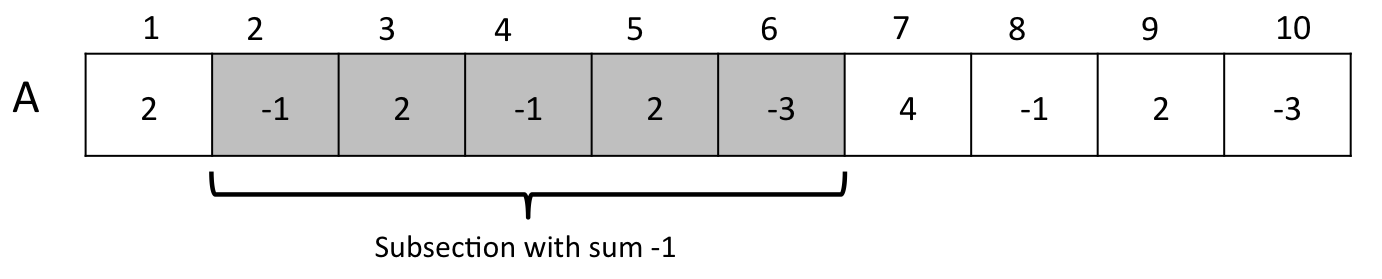
\includegraphics[scale=0.23]{embed/subsection}
\end{figure}

%\vspace{-0.2in}

Let us call a subsection that maximizes the sum of integers, a {\it maximum subsection}. Design a DP algorithm for this problem that output the sum of numbers in a maximum subsection.




%\vspace{0.3in}

\begin{solution}
\paragraph{Description Of Subproblem}
For this problem we define $dp[i]$ to be the answer to the subproblem $S(i)$ where $i \in \{1,2,...n\}$. This subproblem $S(i)$ represents maximum sum of integers in any (non-empty) contiguous subsection that ends at $i^{th}$ element in the array.

To solve the given problem, we shall consider two cases: one where the maximum sum of any subsection is achieved for a non-empty subarray, and the other when it is achieved for an empty subarray.

\paragraph{Base Case}
$dp[1]=A[1]$, as there is only one subsection possible which can end at $1^{st}$ element, which is the array of size 1 containing the element itself.

\paragraph{Recursive Steps} 
\[
        dp[i] = \max
        \begin{cases}
            A[i]\\
            dp[i-1]+A[i] 
        \end{cases}
        \quad \text{ for } i > 1
\]
Suppose we have calculated the $dp[i-1]$ beforehand, and that it gives the solution to $S(i-1)$ correctly. Now we will show that using the above definition of recursive case $dp[i]$ will also calculate the solution to $S(i)$ correctly.
\begin{proof}
Let the size of the subsection with the maximum sum ending at $i^{th}$ index be $k$, then it can be described exhaustively by two cases as shown below.
\begin{enumerate}
    \item \textbf{Case 1} $k = 1$
    \newline There is only one subsection possible of size 1 ending at $i^{th}$ index which is array containing the element itself. In this case the sum of the array would be just $A[i]$.
    \item \textbf{Case 2} $k>1$
    \newline Now as the size of the subsection is greater than 1, and as by the definition of subsection it is contiguous sequence of indices in the array. Therefore the subsection in this case can be considered as the appending the $i^{th}$ element to a subsection ending at $(i-1)^{th}$. 
    \newline Now the maximum subsection possible for the case will be the maximum sum of $A[i]$ and any subsection ending at $(i-1)^{th}$. As the first one is constant it comes down to the maximizing the latter one, whose maximum achievable value is nothing other than the maximum subsection ending at $(i-1)^{th}$ index which is already calculated by $dp[i-1]$ (as assumed above). 
    \newline So the maximum subsection for this case would be just $dp[i-1]+A[i]$
\end{enumerate}

Now as the above cases are exhaustive and mutually exclusive therefore the maximum subsection would fall in one of two cases above. So we will just compute the answer for both the cases (finding maximum over all length 1 subarrays as well as length $> 1$ subarrays) and take the maximum of both of them.
\end{proof}
\paragraph{Order of subproblems solved}
The subproblems will be solved in the increasing order of $i$. That is $S(i)$ is solved before $S(i')$, if $i<i'$.
\begin{gather*}
    dp[1]\; dp[2] \; dp[3] \; \ldots \; dp[n] 
\end{gather*}
We can see from our recursive formulation of the subproblems that subproblem $dp[i]$ depends only on $A[i]$ and $dp[i-1]$, therefore such an ordering is consistent.
\paragraph{Output}
The problem asks for subsection with the maximum sum. Now either the maximum subsection is empty or non empty. For the former one sum is just $0$, for the later one if it ends at index $i$ then in that case the sum would be $dp[i]$. So the maximum sum of any subsection would be just the maximum of both the cases (maximum sum of an empty subsection and the maximum sum of any non-empty subsection). \nl
$output= \max(0,dp[1],dp[2],\ldots, dp[n])$
\paragraph{PseudoCode}
\begin{algorithmic}[1]
\Function{FindMaxSumSubsection}{$A[1 \ldots n]$}
    \If {$n=0$}
        \State \Return 0
    \EndIf
    \State let $dp[1 \ldots n] \gets$ a empty array of size n
    \State  $dp[1] \gets A[1] $
    \For{$i \in [2 \ldots n]$}
            \State $dp[i] \gets \max(A[i],dp[i-1]+A[i])$
    \EndFor
    \State output$\gets$0
    \For{$i \in [1 \ldots n]$}
            \State $output \gets \max(output,dp[i])$
    \EndFor
    \State \Return output
\EndFunction
\end{algorithmic}
\paragraph{Runtime Analysis}
In our algorithm we first initialize the array of size $n$, this will take $O(n)$ time. Now then we just initialize our base case $dp[1]$ which takes $O(1)$ time. Then we fill the array dp in bottom up manner, by iterating using a for loop (line 7-9). This takes $O(n)$ time. Now to find the final answer to the algorithm we have take the max over all $dp[i]$ and 0, by using a for loop. This will also take $O(n)$ time (line 11-13). So the overall runtime complexity of our algorithm would be just $O(n)$.
\paragraph{Small Example}
Let us consider the example given in the problem itself,
\begin{figure}[H]
\centering
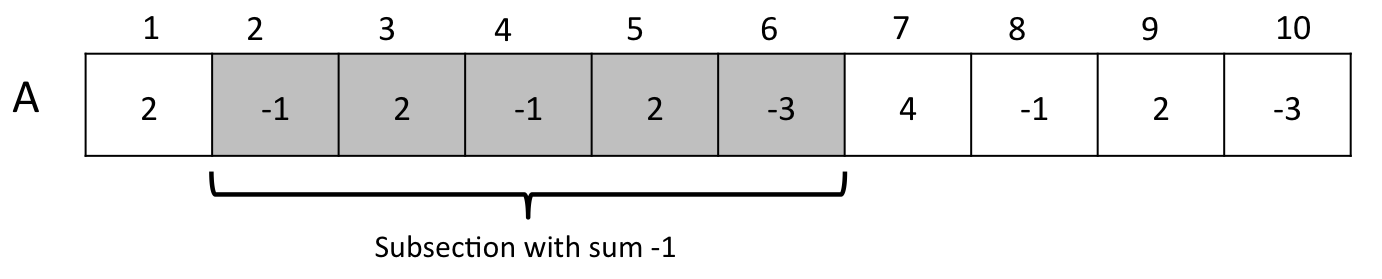
\includegraphics[scale=0.23]{embed/subsection}
\end{figure}
 \begin{center}
        \begin{tabular}{|c|c|c|c|c|c|c|c|c|c|c|}
            \hline
            $i \rightarrow$  & 1 & 2 & 3 & 4 & 5 & 6 & 7 & 8 & 9 & 10  \\
            \hline
             & 2 & 1 & 3 & 2 & 4 & 1 & 5 & 4 & 6 & 3 \\
            \hline
        \end{tabular}
    \end{center}
The second row of above table is our dp array filled in top down manner. 
\newline For the maximum subsection it would be max of whole array and 0 which would be 6, which is in fact the maximum subsection achievable for the above array.

\end{solution}

\question[20] Let $p(1),\dots,p(n)$ be prices of a stock for $n$ consecutive days. 
A $k$-block strategy is a collection of $m$ pairs of days $(b_1,s_1),\dots,(b_m,s_m)$ with $0\leq m \leq k$ and $1\leq b_1<s_1<\dots<b_m<s_m\leq n$. 
For each pair of days $(b_i, s_i)$, the investor buys $100$ shares of stock on day $b_i$ for a price of $p(b_i)$ and then sells them on day $s_i$ for a price of $p(s_i)$ with a total return of:
$$100\sum_{1\leq i \leq m}p(s_i)-p(b_i)$$
Design a DP algorithm that takes as input a positive integer $k$ and the prices of the $n$ consecutive days, $p(1),\dots,p(n)$ and computes the maximum return among all $k$-block strategies.

\begin{solution}
\paragraph{Description Of Subproblem}
For this problem we will define following 2 subproblems. In definition we have used the word ``transaction'' to mean either buying or selling of a stock.
\begin{enumerate}
    \item $ProfitBuy(i, j)$ where $i \in \{1 \ldots n\}$ and $j \in \{1 \ldots k\}$. This sub-problem represents maximum profit that can be obtained \emph{till} day $i$ given that the last transaction in this interval was a ``buy'' transaction and that we have bought \emph{atmost} $j$ stocks.
    \item $ProfitSell(i, j)$ where $i \in \{1 \ldots n\}$ and $j \in \{0 \ldots k\}$. This sub-problem represents maximum profit that can be obtained \emph{till} day $i$ given that the last transaction \textbf{(if any)} in this interval was a ``sell'' transaction and that we have bought \emph{atmost} $j$ stocks.
\end{enumerate}
We remark that while both the subproblems are similar in appearance there are subtle differences between them. First is of course that in $ProfitBuy$ the last transaction is supposed to be a buy transaction and vice versa in $ProfitSell$. Secondly, $ProfitSell$ is also defined for $j = 0$. Thirdly, $ProfitBuy$ requires that there exists a last transaction whereas $ProfitSell$ does not have any such requirement.

Lastly, we will use the notation $ProfitBuy[i,j]$ to denote the answer to the subproblem $ProfitBuy(i,j)$ and similarly for $ProfitSell$.

\paragraph{Base Case}
\begin{enumerate}
    \item $ProfitBuy[1, j] = -100 \cdot p[1] \; \forall j \geq 1$. Since by definition of $ProfitBuy$ the last transaction till day $1$ must be a buy, we have to buy the stock at day 1 in this base case.
    \item $ProfitSell[1, j] = 0 \; \forall j \geq 1$. Since we could not possibly have bought a stock before day 1, therefore we can not sell any stock at day 1.
    \item $ProfitSell[i, 0] = 0 \; \forall i$. If $j=0$ it means that we have not bought any stocks and therefore we can not attempt to sell either.
\end{enumerate}
\paragraph{Recursive Step}
As we have defined 2 subproblems we will therefore also define 2 rules of recursion, one for each subproblem.
\begin{enumerate}
    \item
    \[
        ProfitBuy[i, j] = \max
        \begin{cases}
            ProfitBuy[i-1, j]\\
            ProfitSell[i-1, j-1] - 100 \cdot p[i]
        \end{cases}
        \quad i,j > 1
    \]
    Suppose that we have already computed $ProfitBuy[i-1, j]$ and $ProfitSell[i-1, j-1]$ and they agree with their respective definitions. Then we will show that this expression correctly computes the value $ProfitBuy[i, j]$ in the sense that it agrees with its definition.
    \begin{proof}
    First we will make exhaustive cases on our decision on day $i$. Note that since the last transaction till day $i$ must be a ``buy'' transaction, we only have 2 choices on day $i$ -- do nothing or buy.
    \begin{enumerate}
        \item \textbf{Case 1}. We choose to do nothing (neither buy nor sell the stock) on day $i$. Then, our profit till day $i$ will be the same as our profit till day $i-1$. And to maximise our profit we need to maximise our profit till day $i-1$. Further, since we did not buy any new stock, we will attempt to maximise the profit till day $i-1$ given that we can buy atmost $j$ stocks. This is same as the subproblem $ProfitBuy(i-1, j)$ which, as we assumed, we have already correctly computed.
        \item \textbf{Case 2}. We choose to buy the stock on day $i$. Since by problem constraints we can only buy after we sell the currently holding stock, this means that we must have bought (and sold) atmost $j-1$ stocks till day $i-1$. And, since we are buying the stock at day $i$ we must definitely invest $100 \cdot p[i]$ money in this transaction. So, then to maximise our profits we need to have to make optimal decisions till day $i-1$ which translates to solving the subproblem $ProfitSell(i-1, j-1)$.
    \end{enumerate}
    Clearly, to maximise our profits we will choose the best of the above 2 cases. That is, we will compute answer for both the cases and take the maximum of the two.
    \end{proof}
    \item
    \[
        ProfitSell[i, j] = \max
        \begin{cases}
            ProfitSell[i-1, j]\\
            ProfitBuy[i-1, j] + 100 \cdot p[i]
        \end{cases}
        \quad i,j > 1
    \]
    Suppose that we have already computed $ProfitSell[i-1, j]$ and $ProfitBuy[i-1, j]$ and they agree with their respective definitions. Then we will show that this expression correctly computes the value $ProfitSell[i, j]$ in the sense that it agrees with its definition.
    \begin{proof}
    First we will make exhaustive cases on our decision on day $i$. Note that since the last transaction till day $i$ must be a ``sell'' transaction, we only have 2 choices on day $i$ -- do nothing or sell.
    \begin{enumerate}
        \item \textbf{Case 1}. We choose to do nothing (neither buy nor sell the stock) on day $i$. Then, our profit till day $i$ will be the same as our profit till day $i-1$. And to maximise our profit we need to maximise our profit till day $i-1$. Further, since we did not buy any new stock, we will attempt to maximise the profit till day $i-1$ given that we can buy atmost $j$ stocks. This is same as the subproblem $ProfitSell(i-1, j)$ which, as we assumed, we have already correctly computed.
        \item \textbf{Case 2}. We choose to sell the stock on day $i$. We can only sell a stock if we are holding one. This means that if we have chosen to sell the stock on day $i$, then our last transaction must have been a ``buy'' transaction. Further, by selling the stock we will gain $100 \cdot p[i]$ regardless of when did we buy the stock. So to maximise our profits till day $i$ we must maximise our earnings till day $i-1$ which translates to solving the subproblem $ProfitBuy(i-1, j)$ which, as we have assumed, is already correctly computed.
    \end{enumerate}
    Clearly, to maximise our profits we will choose the best of the above 2 cases. That is, we will compute answer for both the cases and take the maximum of the two.
    \end{proof}    
\end{enumerate}
\paragraph{Order in which sub-problems are solved}
We will solve the subproblems in increasing order of $i$, and for same $i$ in increasing order of $j$. More specifically, the subproblem $(i, j)$ is solved before $(i', j')$ \emph{iff} $i < i'$ or $i = i'$ and $j < j'$.
\begin{gather*}
    ProfitBuy(2, 1) \; ProfitSell(2, 1) \; \ldots \; ProfitBuy(2, k) \; ProfitSell(2, k) \\
    \vdots\\
    ProfitBuy(n, 1) \; ProfitSell(n, 1) \; \ldots \; ProfitBuy(n, k) \; ProfitSell(n, k)
\end{gather*}
We can see from our recursive formulation of the subproblems that subproblem $(i, j)$ depends only on subproblems $(i-1, j-1)$ or $(i-1, j)$ both of which precede the subproblem in this order. Therefore such an ordering of subproblems is consistent.
\paragraph{Output}
The problem asks to compute maximum profit obtainable if we can buy atmost $k$ stocks in $n$ days. Further, our last transaction must have been a ``sell'' transaction as we also need to sell all the stocks that we have bought. This corresponds to solving the subproblem $ProfitSell(n, k)$ in our formulation.
\paragraph{Algorithm}
\begin{algorithmic}[1]
\Function{FindMaxProfit}{$p[1 \ldots n]$, $k$}
    \State let $ProfitBuy[1 \ldots n][1 \ldots k] \gets$ a empty table of size $n \times k$
    \State let $ProfitSell[1 \ldots n][0 \ldots k] \gets$ a empty table of size $n \times (k+1)$
    \For{$j \in [1 \ldots k]$}
        \State $ProfitBuy[1][j] \gets -100 * p[1]$
        \State $ProfitSell[1][j] \gets 0$
    \EndFor
    \For{$i \in [1 \ldots n]$}
        \State $ProfitSell[i][0] \gets 0$
    \EndFor
    \For{$i \in [2 \ldots n]$}
        \For{$j \in [1 \ldots k]$}
            \State $ProfitBuy[i][j] \gets \max(ProfitBuy[i-1][j], ProfitSell[i-1][j-1] - 100 * p[i])$
            \State $ProfitSell[i][j] \gets \max(ProfitSell[i-1][j], ProfitBuy[i-1][j] + 100 * p[i])$
        \EndFor
    \EndFor
    \State \Return $ProfitSell[n][k]$
\EndFunction
\end{algorithmic}
\paragraph{Runtime Analysis}
In our algorithm first we initialize 2 tables of sizes $n \times k$ and $n \times (k+1)$ respectively. Both of these operations will take $O(nk)$ time. Then we have a initialization loop which has $O(k)$ iterations and in each iteration we do a $O(1)$ computation and memory access. Then again we have a initialization loop which similarly does $O(n)$ iterations. Finally we have the update loop which is a nested loop. The outer loop runs $n-1$ times and the inner loop runs $k$ times. In the body of inner loop we again do $O(1)$ memory accesses and $O(1)$ computations so in total the nested loop will take $O(nk)$ time. So the runtime complexity of our algorithm is $O(nk)$.
\paragraph{Example}
For example suppose we are given $p = [1, 0, 1, 2]$ and $k = 2$. First in our algorithm we will initialize the tables $ProfitBuy$ and $ProfitSell$ as
\[
    ProfitBuy =
    \begin{bmatrix}
    -100 & -100 \\
    - & - \\
    - & - \\
    - & - \\
    \end{bmatrix} \quad
    ProfitSell =
    \begin{bmatrix}
    0 & 0 & 0 \\
    0 & - & - \\
    0 & - & -\\
    0 & - & - \\
    \end{bmatrix}
\]
After first step,
    \[
        ProfitBuy(2, j) = \max
        \begin{cases}
            ProfitBuy(1, 1)\\
            ProfitSell(1, j-1) - 100 \cdot p[2]
        \end{cases}
        =
        \begin{cases}
            -100\\
            0 - 100 \cdot 0
        \end{cases}
        = 0
    \]
    \[
        ProfitSell(2, j) = \max
        \begin{cases}
            ProfitSell(1, j)\\
            ProfitBuy(1, j-1) + 100 \cdot 0
        \end{cases}
        =
        \begin{cases}
            0\\
            -100 + 100 \cdot 0
        \end{cases}
        = 0
    \]
\[
    ProfitBuy =
    \begin{bmatrix}
    -100 & -100 \\
    0 & 0 \\
    - & - \\
    - & - \\
    \end{bmatrix} \quad
    ProfitSell =
    \begin{bmatrix}
    0 & 0 & 0 \\
    0 & 0 & 0 \\
    0 & - & -\\
    0 & - & - \\
    \end{bmatrix}
\]
And so on we can complete the tables ...
\[
    ProfitBuy =
    \begin{bmatrix}
    -100 & -100 \\
    0 & 0 \\
    0 & 0 \\
    0 & 0 \\
    \end{bmatrix} \quad
    ProfitSell =
    \begin{bmatrix}
    0 & 0 & 0 \\
    0 & 0 & 0 \\
    0 & 100 & 100\\
    0 & 200 & 200 \\
    \end{bmatrix}
\]
The answer is then $ProfitSell[4][2] = 200$ which is correct.

\end{solution}



%\vspace{0.3in}



\question[20] You are given an $n \times 5$ matrix $A$ consisting of integers (positive or negative). 
Your goal is to find a set $S$ of tuples $(i, j)$ indicating locations of the 2-D matrix $A$ such that:
\begin{enumerate}
\item $\sum_{(i, j) \in S} A[i, j]$ is maximized, and
\item For all pairs of tuples $(i_1, j_1), (i_2, j_2) \in S$, $(i_2, j_2) \notin \{(i_1-1, j_1), (i_1+1, j_1), (i_1, j_1-1), (i_1, j_1+1)\}$.
\end{enumerate}

({\it For example, consider the $2 \times 5$ matrix below. The set of locations that satisfies (1) and (2) above are indicated by shading these locations in the matrix.})

\begin{figure}[h]
\centering
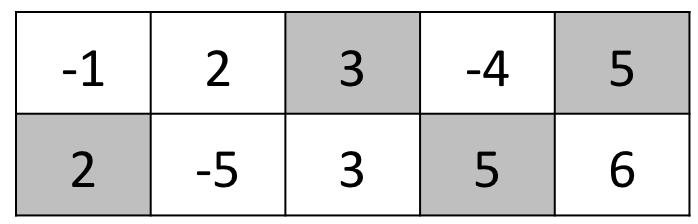
\includegraphics[scale=0.2]{embed/array}
\end{figure}

Design a DP algorithm for this problem that outputs the maximum possible sum attainable.

%%\vspace{0.3in}

\begin{solution}
For the sake of convenience, we first enumerate all possible subsets $S$ of $\{1, 2, 3, 4, 5\}$ which have the following property: For any $x \in S$, $\{x - 1, x + 1\} \cap S = \emptyset$ (i.e., no two consecutive integers are in $S$). \nl
These sets are $\emptyset, \{1\}, \{2\}, \{3\}, \{4\}, \{5\}, \{1, 3\}, \{1, 4\}, \{1, 5\}, \{2, 4\}, \{2, 5\}, \{3, 5\}, \{1, 3, 5\}$.\nl
Call this collection of sets $I$ (we will treat this as an array of sets for the remaining solution).\nl
Now coming to the format of the main proof:
\begin{enumerate}
\item Subproblems\nl
$P(i, S) = $ the maximum possible sum attainable when the set of tuples is restricted to rows $1\ldots i$, and precisely those elements of row $i$ are chosen that have their column indices in $S$. ($S$ can be empty).
\item Base case\nl
The base case is when $i = 0$. For any set $S$ of indices, the value of $P(0, S)$ is vacuously $0$.
\item Recursion with justification\nl
Consider the problem to which $P(i, S)$ is the answer. In such a problem, we restrict the choices of pairs of indices to those which have row numbers in $\{1, \cdots, i\}$.\nl
Note that the set of column indices that can be chosen at row $i$ in a solution to this problem is in $I$ (and each set in $I$ is a valid choice for the indices chosen in row $i$, disregarding the
choices of indices for the previous row). Note that for any choice $S$ of indices in row $i$, for a valid choice $T$ of the previous row, we must have $S \cap T = \emptyset$, and the converse holds true as well.\nl
Suppose there is a choice $W$ of tuples of indices which have row indices at most $i$, with the row $i$ column index set being $S$ and row $i - 1$ column index set being $T$, which has a sum more than $P(i - 1, T) + \sum_{j \in S} A[i, j]$. Then $W \setminus \{(i, j) \mid j \in S\}$ is a choice of tuples of indices which have row indices at most $i - 1$, but it the sum of elements corresponding to that choice of indices exceeds $P(i - 1, T)$, which is impossible by the definition of $P$. Hence, for any choice $W$ as mentioned, the sum of chosen row $i$ elements + $P(i - 1, T)$ must be an upper bound for the sum corresponding to $W$. The maximum of this expression over all $T$ is thus an upper bound on $P(i, S)$. However, note that this is achievable as well (merely choose the $T$ corresponding to the maximum).\nl
Hence, the answer to the problem is (for $i > 0$):
\begin{align*}
    P(i, S) &= \max_{T \in I, S \cap T = \emptyset} \left(P(i - 1, T) + \sum_{j \in S} A[i, j]\right)\\
            &= \left(\max_{T \in I, S \cap T = \emptyset} P(i - 1, T)\right) + \left(\sum_{j \in S} A[i, j]\right)
\end{align*}
where the second equality holds because the sum doesn't depend on $T$.\nl
Note that for any set in $I$, there is at least one disjoint set in $I$ (for instance, the empty set), and hence the max is not empty.
\item Order in which sub-problems are solved\nl
We solve the problems in the following order:\nl
If $i < j$, then problem $(i, S)$ is solved before $(j, T)$ for any $S, T \in I$. If $i = j$, then problem $(i, S)$ is solved before $(j, T)$ if and only if $S$ comes before $T$ in $I$. Note that this is a valid order of solving the subproblems since the expression of the answer to $(i, S)$ contains the answers to problems of the form $(i - 1, T)$ for some $T$, and all of these are computed before we compute $P(i, S)$.
\item Form of output\nl
The DP table of the algorithm will be in the form of a matrix $D$, where $D[i, j]$ denotes $P(i, I_j)$, where $I_j$ is the set at index $j$ in the array $I$. Note that this is 0-indexed, as is $I$, however we assume that $A$ is 1-indexed.

The output will be an integer, and will be the maximum of $D[n, j]$ over all $j$ where $j$ ranges from $0$ to $12$ (all indices of $I$).

\item Pseudocode

\begin{algorithmic}[1]
    \Function{MaxSum}{$A, n$}
        \State \textbf{let} $D := $ new 2D array of dimension $(n + 1, 13)$, initialised to all $0$s.
        \For{$i \in \{1 \ldots n\}$}
            \For{$j \in \{0 \ldots 12\}$}
                \For{$k \in \{0 \ldots 12\}$}
                    \If{$I_j \cap I_k = \emptyset$}
                        \State $D[i, j] := \max(D[i, j], D[i - 1, k])$
                    \EndIf
                \EndFor
                \For{$l \in I_j$}
                    \State $D[i, j] := D[i, j] + A[i, l]$
                \EndFor
            \EndFor
        \EndFor
        \State \textbf{let} $s = 0$
        \For{$j \in \{0 \ldots 12\}$}
            \State $s := \max(s, D[n, j])$
        \EndFor
        \State \Return $s$
    \EndFunction
\end{algorithmic}

\item Runtime analysis

    Initializing $D$ takes $\Theta(n)$ time. Checking for intersection at line 6, as well as taking the max at line 7, takes $\Theta(1)$ time. Hence one iteration of the loop starting at line $5$
    takes $\Theta(1)$ time. The loop at line 10 takes $\Theta(1)$ time, and since the loop at line $4$ takes $\Theta(1)$ time, one iteration of the loop starting at line $4$ takes $\Theta(1)$ time.
    Hence the loop starting at line $3$ takes $\Theta(n)$ time. Lines 15-19 take $\Theta(1)$ time, and hence the overall time complexity is $\Theta(n)$.

\item Small example

    The matrix $D$ for the mentioned example in the problem is as follows:
    \begin{center}
        \begin{tabular}{|c|c|c|c|c|c|c|c|c|c|c|c|c|c|c|}
            \hline
            $i \downarrow, j \rightarrow$ & 0 & 1 & 2 & 3 & 4 & 5 & 6 & 7 & 8 & 9 & 10 & 11 & 12 \\
            \hline
            0 & 0 & 0 & 0 & 0 & 0 & 0 & 0 & 0 & 0 & 0 & 0 & 0 & 0\\
            \hline
            1 & 0 & -1 & 2 & 3 & -4 & 5 & 2 & -5 & 4 & -2 & 7 & 8 & 7\\
            \hline
            2 & 8 & 10 & 3 & 10 & 13 & 9 & 12 & 15 & 11 & 8 & 4 & 11 & 13\\
            \hline
        \end{tabular}
    \end{center}

    From reading off the last row, the answer is $15$.

\end{enumerate}

\end{solution}

\question[20] A town has $n$ residents labelled $1, ..., n$. 
All $n$ residents live along a single road. The town authorities suspect a virus outbreak and want to set up $k$ testing centers along this road. 
They want to set up these $k$ testing centers in locations that minimises the sum total of distance that all the residents need to travel to get to their nearest testing center. 
You have been asked to design an algorithm for finding the optimal locations of the $k$ testing centers.

Since all residents live along a single road, the location of a resident can be identified by the distance along the road from a single reference point (which can be thought of as the starting point of the town). 
As input, you are given integer $n$, integer $k$, and the location of the residents in an integer array $A[1...n]$ where $A[i]$ denotes the location of resident $i$. Moreover, $A[1] \leq A[2] \leq A[3] \leq ... \leq A[n]$. Your algorithm should output an integer array $C[1...k]$ of locations such that the following quantity gets minimised: 
\[
\sum_{i=1}^{n} D(i), \textrm{ where } D(i) = \min_{j \in \{1, ..., k\}}{\lvert A[i] - C[j] \rvert}
\]
Here $\lvert x - y \rvert$ denotes the absolute value of the difference of numbers $x$ and $y$. Note that $D(i)$ denotes the distance resident $i$ has to travel to get to the nearest testing center out of centers at $C[1], ..., C[k]$.

%\vspace{0.1in}

({\it For example, consider $k = 2$ and $A = [1, 2, 3, 7, 8, 9]$. A solution for this case is $C = [2, 8]$. Note that for testing centers at locations $2$ and $8$, the total distance travelled by residents will be $(1 + 0 + 1 + 1 + 0 + 1) = 4$.})

%\vspace{0.1in}

Design a DP algorithm for this problem that outputs the minimum achievable value of the total distance.


%\vspace{0.3in}

\begin{solution}
First we finish off the case where $k$ is at least the number of distinct resident locations. Then we can choose a testing center at all possible locations of a resident, and assign arbitrary locations to the remaining testing centers, to get $\sum_{i = 1}^n D(i) = 0$, which is the minimum possible value of the quantity on the LHS since $D$ is non-negative.

Henceforth, we shall assume that $k$ is less than the number of distinct resident locations.

We will need a few preliminaries before proceeding to the main solution.

Firstly, we will show a lemma about sum of absolute values.

\begin{lemma}
    A number $x$ is said to be a median of a sorted sequence $a_1, a_2, \ldots, a_n$ if either
    \begin{enumerate}
        \item $n$ is odd, and $x = a_{\frac{n - 1}{2}}$, or
        \item $n$ is even, and $x \in \left[a_{\frac{n}{2}}, a_{\frac{n}{2} + 1}\right]$.
    \end{enumerate}
    Then the function $f : \mathbb{R} \to \mathbb{R}$ defined by $f(x) = \sum_{i = 1}^n |x - a_i|$ 
    \begin{enumerate}
        \item Achieves its minimum, and
        \item The set of values at which it achieves its minimum is precisely the set of medians of $a_1, a_2, \ldots, a_n$.
    \end{enumerate}
\end{lemma}
\begin{proof}
    This function is a piecewise linear continuous function. We have three cases for where $x$ can lie:
    \begin{enumerate}
        \item $x \le a_1$: In this case, we have $|x - a_i| = a_i - x$ for all $i$, and thus this function is decreasing in this interval.
        \item $x \ge a_n$: In this case, we have $|x - a_i| = x - a_i$ for all $i$, and the function is increasing in this interval.
        \item $a_j \le x \le a_{j + 1}$: In this case, we have $|x - a_i| = x - a_i$ for $i \le j$ and $|x - a_i| = a_i - x$ for $i > j$. Hence, the coefficient of $x$ in this interval is $j - (n -
            j) = 2j - n$. Hence, depending on whether $2j - n$ is $<, =$ or $> 0$, the function is decreasing, constant and increasing in this interval.
    \end{enumerate}

    From here, we come to know that the function is decreasing on the interval $\left(-\infty, a_{\left\lceil\frac{n}{2}\right\rceil}\right]$ and increasing on the interval
    $\left[a_{\left\lfloor\frac{n}{2}\right\rfloor + 1}, \infty\right)$, and constant on the remaining interval (if any). This completes the proof of the lemma.
\end{proof}

Consider any $A$ and an array $C$ of locations (in sorted order). Define $L(i)$ to be the index of the location in $C$ closest to $A[i]$. In case of ties, choose the least such index.\\

\begin{claim}
For any $i < j$, we have $L(i) \le L(j)$.
\end{claim}
\begin{proof}
If $A[i] = A[j]$, we are done. Henceforth assume $A[i] < A[j]$. 

Suppose $L(i) > L(j)$. We make the following cases:

\begin{enumerate}
\item $C[L(i)] \le A[j]$: In this case, $C[L(i)]$ is closer to $A[j]$ than $C[L(j)]$ (by the sorted-ness of $C$), which is a contradiction.
\item $A[j] < C[L(i)]$: Note that $A[i] < A[j] < C[L(i)]$, and $C[L(j)] < C[L(i)]$.
    We make two subcases:
        \begin{enumerate}
            \item $A[i] \le C[L(j)]$: In this case, $A[i]$ is closer to $C[L(j)]$ than $C[L(i)]$, which is a contradiction.
            \item $A[i] > C[L(j)]$: In this case, $C[L(j)], A[i], A[j], C[L(i)]$ are in this order. Let $D(i), D(j)$ be as defined, and let $D'(i), D'(j)$ be the distance from $A[i], A[j]$ to
                $C[L(j)], C[L(i)]$ respectively. Then we have $D(i) + D(j) = D'(i) + D'(j) + |A[i] - A[j]| > D'(i) + D'(j)$. However, by the definition of $D$, we have $D(i) \le D'(i)$, $D(j) \le D'(j)$, adding which gives a contradiction.
        \end{enumerate}
\end{enumerate}
    Hence in all cases, $L(i) > L(j)$ leads to a contradiction, which completes the proof.
\end{proof}

Note that this implies that we can partition the array $A$ into contiguous chunks, each of which have the same value of $L(i)$.

Consider any optimal solution, and each chunk in it. Note that there will be at most $k$ chunks.

\begin{claim}
The number of chunks is precisely $k$.
\end{claim}
\begin{proof}
    Suppose that this is not the case. Then since $k$ is less than the number of distinct positions of residents, there exists at least one location among $A[1], \ldots, A[n]$ which doesn't have a
    testing center on it, and since there are less than $k$ chunks, there is at least one testing center that is not associated to a chunk. If we assign all the unassigned testing centers to that location, the term corresponding to that location
    strictly decreases to 0, and none of the other terms can increase, which leads to a contradiction.
\end{proof}

\begin{claim}
In any optimal solution, the chosen value of $C$ corresponding to each chunk is one of the medians of each chunk (a median is as defined above, and not the usual definition of a median).
\end{claim}
\begin{proof}

    From the previous claim, we know that there are precisely $k$ chunks, and the $i^\mathrm{th}$ chunk corresponds to $C[i]$ (since $C$ is sorted). 

    Let the starting index of $j^\mathrm{th}$ chunk be $i_j$, and define $i_{k + 1} = n + 1$.

    We shall construct a solution by replacing $C[j]$ by $C'[j]$, which is defined as one of the medians of $A[i_j], \ldots, A[i_{j + 1} - 1]$.

    Note that for each $A[i]$ for $i \in \{i_j, \ldots, i_{j+1}-1\}$, if the new $D-$function is $D'$, then we have $D'(i) \le |A[i] - C'[i]|$.

    By the optimality of $C$, we have
    $$\sum_{i = 1}^n |A[i] - C[i]| = \sum_{i = 1}^n D(i) \le \sum_{i = 1}^n D'(i) \le \sum_{i = 1}^n |A[i] - C'[i]|$$

    However, for each chunk, applying the lemma gives us that 
    $$\sum_{i = i_j}^{i_{j+1} - 1} |A[i] - C[i]| \le \sum_{i = i_j}^{i_{j+1} - 1} |A[i] - C'[i]|$$

    Combining these two, we note that equality must hold, and hence for each chunk, $C[i]$ must achieve the minimum of the sum for that chunk, which implies that it must be one of the medians of the chunk, by the lemma.
\end{proof}

Hence this shows that we now only need to focus on chunks of the array $A$ and their medians, i.e., if we focus solely on partitions of $A$, we can simply assign each partition its median, and since
the optimal $C$ will have each element as a median of its associated chunk, the best possible solution must also be of this form.\\

Hence for the case where $k$ is less than the number of distinct elements in $A$, we shall focus our attention to the following problem instead:

{\bf
For an array $A$, find a partition of $A$ into $k \ge 1$ contiguous subarrays $A[i_1\ldots i_2 - 1], \ldots, A[i_k\ldots i_{k+1} - 1]$, such that the following quantity is minimized:

$$V(A, \{i_1, \ldots, i_k\}) = \sum_{j = 1}^k \sum_{i = i_j}^{i_{j+1} - 1} |A[i] - \text{median}(A[i_j\ldots i_{j+1} - 1])| $$

and return the value of this quantity (here $i_{k+1} = n + 1$ as defined earlier).
}

Now we come back to the main problem. 

Note that we have shown that in case of an array with $w$ distinct elements, and $n$ total elements, and $k < w$, all chunks will have a bijective correspondence with $C$, and the
corresponding $C-$value is a median.

If $w \le k \le n$, we can always find an assignment which has non-empty chunks of equal elements, and their corresponding $C$-values would be their medians, and this gives the value of that partition to be $0$.

If $k > n$, we can keep adding arbitrary elements of the array $A$ to $C$ after doing the above to give the answer $0$.

Hence this completes the analysis for the problem.

We shall need some preprocessing to be able to compute the contribution of a chunk efficiently.

Note that using our definition of a median, the middle element of an odd-sized array is a median, and the left-middle element of an even-sized array is a median. More formally, note that in a
sorted subarray $A[i\ldots j]$, $A[\lfloor(i + j) / 2\rfloor]$ is a median.

Define $Cost(A, i, j)$ to be the contribution of the elements from a chunk $A[i\ldots j]$ when we assign the median to it.

Also define the prefix sums $p[i]$ to be the sum of $A[1\ldots i]$, and $p[0] = 0$. Then the sum of $A[i\ldots j]$ is $p[j] - p[i - 1]$.

Then we have 
$$Cost(A, i, j) = \sum_{k = i}^{\lfloor(i + j)/2\rfloor} (A[\lfloor(i + j) / 2\rfloor] - A[k]) + \sum_{k = \lfloor(i + j)/2\rfloor + 1}^{j} (A[k] - A[\lfloor(i + j)/2\rfloor])$$

If $i + j$ is even, then this reduces to (after discarding the middle element and cancelling the remaining instances of $A[(i + j)/2]$):

$$\sum_{k = (i + j)/2 + 1}^j A[k] - \sum_{k = i}^{(i + j) / 2 - 1} A[k] = p[j] - p[(i + j) / 2] - p[(i + j) / 2 - 1] + p[i - 1]$$

If $i + j$ is odd, then a similar reduction gives 

$$\sum_{k = (i + j + 1)/2}^j A[k] - \sum_{k = i}^{(i + j - 1) / 2} A[k] = p[j] - p[(i + j - 1) / 2] - p[(i + j - 1) / 2] + p[i - 1]$$

Thus from here, we note that $Cost(A, i, j) = p[j] - p[m] - p[m'] + p[i - 1]$ where $m' = \lfloor(i + j - 1)/2\rfloor$ and $m = \lceil(i + j - 1)/2\rceil$.

\begin{enumerate}

\item Subproblems

We will have the following subproblems:

        $P(i, j):$ Find the minimum possible value of $V(A[1\ldots i], \{i_1, \ldots, i_j\})$, say $Opt(i, j)$ if $j$ is less than the number of distinct elements in $A[1\ldots i]$, 0 otherwise. Here $i \in \{0, 1, \ldots, n\}$ and $j \in \{1, 2, \ldots, k\}$. $j = 0$ is invalid since we have to put at least one element in the array $C$ for the $\min$ in the definition to be well-defined.

\item Base case

    \begin{enumerate}
    %The first types of base cases will be when $j \ge i$: in this case, the answer is $0$.
    \item When $j = 1$: in this case, the answer is $Cost(A, 1, i)$.
    \item When $i = 0$: in this case, the answer is $0$.
    \end{enumerate}

\item Recursion with justification

        Consider $P(i, j)$ where $j > 1, i \ge 1$.

        Now note that the last partition can start from $i'$ where $1 \le i' \le i$.

        We claim that the answer to this problem is the minimum of $Cost(A, i', i) + Opt(i' - 1, j - 1)$ over all $i'$. 

        For a proof, suppose there is a solution to $P(i, j)$ in which the last chunk has endpoints $i', i$ and has a smaller value. Then we have a solution for $P(A, i' - 1, j - 1)$ which has a lower
        value than $Opt(i' - 1, j - 1)$, contradiction. So $\min_{i' \in \{1, \ldots, i\}} Cost(A, i', i) + Opt(i' - 1, j - 1) \le Opt(i, j)$. Now to construct the solution that achieves the bound,
        let $i'$ be the argmin of the expression. Then we choose the optimal solution for $A[1\ldots i'-1]$ with $j - 1$ partitions and add the partition $A[i' \ldots i]$ to it, so we are done.
        
        Note that in the case when $j$ is at least the number of distinct elements in $A[1\ldots i]$, choosing $i'$ to be the least index the element at which is $A[i]$ leads to the answer $0$ (since the corresponding subproblem has exactly one distinct element less than the current subproblem, and $j$ replaced by $j - 1$), and hence this formula works in this case too.
        
        Hence, we have
        $$Opt(i, j) = \min_{i' \in \{1, \ldots, i\}} \left(Opt(i' - 1, j - 1) + Cost(A, i', i)\right)$$

\item Order in which sub-problems are solved

    We solve the base cases in the order $(i, j) = (1, 1), (2, 1), \ldots, (n, 1), (0, 1), (0, 2), \ldots, (0, k)$.

    We then solve the remaining problems in lexicographical order of $(i, j)$.

    Note that this is a valid order of solving problems because while computing $Opt(i, j)$, we either need a base case or a value computed before it, the pair of indices corresponding to which is lexicographically smaller than $(i, j)$.

\item Form of output

    If $k \ge n$, then we straight up return 0. Else we return $D[n, k]$, where $D$ is the table in the array that we maintain to store the answers to the sub-problems.

\item Pseudocode

    \begin{algorithmic}[1]
        \Function{MinCost}{$A[1\ldots n], k$}
            \If{$k \ge n$}
                \State \Return 0
            \EndIf
            \State \textbf{let} $p[0\ldots n]$ be an array initialized to all 0s
            \For{$i \in \{1\ldots n\}$}
                \State $p[i] := p[i - 1] + A[i]$
            \EndFor
            \Function{Cost}{$i, j$}
                \State \Return $p[j-1]-p[\lfloor(i+j-1)/2\rfloor]-p[\lceil(i+j-1)/2\rceil]+p[i-1]$
            \EndFunction
            \State \textbf{let} $D$ be a 0-indexed 2D array of dimension $(n + 1, k + 1)$ initialized to $\infty$
            \For{$i \in \{1\ldots n\}$}
                \State $D[i, 1] := Cost(1, i)$
            \EndFor
            \For{$j \in \{1\ldots k\}$}
                \State $D[0, j] := 0$
            \EndFor
            \For{$i \in \{1\ldots n\}$}
                \For{$j \in \{2\ldots k\}$}
                    \For{$i' \in \{1\ldots i\}$}
                        \State $D[i, j] := \min(D[i, j], D[i' - 1, j - 1] + Cost(i', i))$
                    \EndFor
                \EndFor
            \EndFor
            \State \Return $D[n, k]$
        \EndFunction
    \end{algorithmic}

\item Runtime analysis

    Note that if $k \ge n$, then the program takes $O(1)$ time.
    Otherwise, we create $p$ in $O(n)$ time, compute it in $O(n)$ time using the loop at line 6, create $D$ in time $O(nk)$ at line $12$. Then we do initialization of base cases in $O(n + k)$ time
    using two loops. Then we have three nested loops. The innermost loop's body
    takes $O(1)$ time to run, since cost can be computed in $O(1)$ using $p$, and the minimum function takes $O(1)$ to run as well. Hence the innermost loop takes time $O(i)$. The outer loop
    runs this $k$ times, so it takes time $O(ik)$. The outermost loop runs once for each $i$, and hence the total time is $O(n^2 k)$ for the outermost loop. The return takes $O(1)$ time. Hence the
    complete algorithm runs in $O(n^2 k)$ time for $k < n$. Thus the complexity of the algorithm is:

    \begin{equation*}
        T(n) \in 
        \begin{cases}
            O(1) & \text{ if } k \ge n \cr
            O(n^2k) & \text{ otherwise} \cr
        \end{cases}
    \end{equation*}

\item Small example

    $(n, k) = (15, 10)$, $A = \{1, 2, 3, 3, 3, 4, 5, 6, 7, 7, 8, 9, 10, 11, 11\}$

    $D$ is as follows:

    \begin{center}
        \begin{tabular}{|c|c|c|c|c|c|c|c|c|c|c|c|}
            \hline
            $i \downarrow, j \rightarrow$ & 0 & 1 & 2 & 3 & 4 & 5 & 6 & 7 & 8 & 9 & 10 \\
            \hline
            0 & $\infty$ & 0 & 0 & 0 & 0 & 0 & 0 & 0 & 0 & 0 & 0 \\
            \hline
            1 & $\infty$ & 0 & 0 & 0 & 0 & 0 & 0 & 0 & 0 & 0 & 0 \\
            \hline
            2 & $\infty$ & 1 & 0 & 0 & 0 & 0 & 0 & 0 & 0 & 0 & 0 \\
            \hline
            3 & $\infty$ & 2 & 1 & 0 & 0 & 0 & 0 & 0 & 0 & 0 & 0 \\
            \hline
            4 & $\infty$ & 3 & 1 & 0 & 0 & 0 & 0 & 0 & 0 & 0 & 0 \\
            \hline
            5 & $\infty$ & 3 & 1 & 0 & 0 & 0 & 0 & 0 & 0 & 0 & 0 \\
            \hline
            6 & $\infty$ & 4 & 2 & 1 & 0 & 0 & 0 & 0 & 0 & 0 & 0 \\
            \hline
            7 & $\infty$ & 6 & 4 & 2 & 1 & 0 & 0 & 0 & 0 & 0 & 0 \\
            \hline
            8 & $\infty$ & 9 & 5 & 3 & 2 & 1 & 0 & 0 & 0 & 0 & 0 \\
            \hline
            9 & $\infty$ & 13 & 6 & 4 & 3 & 2 & 1 & 0 & 0 & 0 & 0 \\
            \hline
            10 & $\infty$ & 17 & 7 & 5 & 3 & 2 & 1 & 0 & 0 & 0 & 0 \\
            \hline
            11 & $\infty$ & 21 & 8 & 6 & 4 & 3 & 2 & 1 & 0 & 0 & 0 \\
            \hline
            12 & $\infty$ & 26 & 10 & 8 & 6 & 4 & 3 & 2 & 1 & 0 & 0 \\
            \hline
            13 & $\infty$ & 31 & 13 & 9 & 7 & 5 & 4 & 3 & 2 & 1 & 0 \\
            \hline
            14 & $\infty$ & 37 & 16 & 10 & 8 & 6 & 5 & 4 & 3 & 2 & 1 \\
            \hline
            15 & $\infty$ & 42 & 19 & 11 & 9 & 7 & 5 & 4 & 3 & 2 & 1 \\
            \hline
        \end{tabular}
    \end{center}

    Note that the column corresponding to $j = 0$ is never used and has a value $\infty$ just because it is never updated (and doesn't correspond to a valid subproblem, as mentioned in the description of the subproblems).

\item Remark: In a private post to instructors on Piazza, I had mentioned that there exists an $O(nk)$ DP solution using the SMAWK algorithm as well, so the above algorithm is not optimal, but as the instructor replied, the exhibited time complexity $O(n^2k)$ qualifies for full credit.

\end{enumerate}

\end{solution}

\question[20] You have a set of $n$ integers $\{x_1, ..., x_n\}$ such that $\forall j, x_j \in \{0, 1, ..., K\}$.
You have to design an algorithm to partition the set $\{1, ..., n\}$ into two disjoint sets $I_1$ and $I_2$ such that such that $|S_1 - S_2|$ is minimized, where $S_1 = \sum_{j \in I_1} x_j$ and $S_2 = \sum_{j \in I_2} x_j$.
Design an algorithm that outputs the minimum value of $|S_1 - S_2|$ achievable.
The running time of your algorithm should be polynomial in $n$ and $K$.
\begin{solution}

\paragraph{Description Of Subproblem}
Let $A$ be an array of size $n$ where $A[i]=x_i$ and $S=\sum_{i}^{n}x_i$. Also $sum(\emptyset)=0$, that is sum of empty set is $0$.\nl
For this problem we define $dp[i][j]$ to be the solution to the subproblem $Sub(i, j)$ where $i \in \{0,1,2,\ldots,n\}$ and $j \in \{0,1,2,\ldots,S\}$. This subproblem $Sub(i, j)$ represents whether it is possible or not to find some subset in array $A[1,2,\ldots,i]$ whose sum is $j$ (and hence $dp$ is a boolean 2D array). Note that for $i=0$ the subset will be found in $A[]$ which is the empty array.
\paragraph{Base Case}
There will be two types of base cases:
\begin{enumerate}
    \item $(i, j) = (0, 0)$. Here $dp[0][0]=True$ as the only subset possible in this case would be $\emptyset$ whose sum is $0$, therefore $0$ sum is achievable in case of $i=0$.
    \item $j = 0, i \in \{1, \ldots, n\}$. Here $dp[i][0]=True$ as we can always take a empty subset therefore sum 0 is always achievable.
    \item $i = 0, j \in \{1, \ldots, S\}$. Here $dp[0][j]=False$, as only subset possible in this case would be $\emptyset$ whose sum is $0$, therefore for $j>0$, $dp[0][j]$ would be False.
\end{enumerate}

\paragraph{Recursive Steps} 
\[
    dp[i][j]=
    \begin{cases}
        dp[i-1][j] & j<A[i]\\
        dp[i-1][j] \text{ or } dp[i-1][j-A[i]] &j\geq A[i]
    \end{cases}
\]
Suppose we have calculated the $dp[i-1][j]$ and $dp[i-1][j-A[i]]$ before hand. Now we will show that using the above definition of recursive case dp[i][j] will also calculated correctly.
\begin{proof}
All the subsets using $A[1,2,..i]$ can be classified exhaustively as the two case below.
\begin{enumerate}
    \item \textbf{Case 1} $A[i]$ is excluded
    \newline As in this case $A[i]$ is excluded all the subset can be considered as the subset formed from $A[1,2,...(i-1)]$. Now to find if the sum j is achievable from the subsets of this case it would be just to find that if it is possible to achieve sum from the subset formed from $A[1,2,...(i-1)]$, which is nothing just $dp[i-1][j]$
    \item \textbf{Case 2} $A[i]$ is included
    \newline As in this case $A[i]$ is included all the subset can be considered as the subset formed from $A[1,2,...(i-1)]$ and adding $A[i]$ to the subset. Now to find if the sum j is achievable from the subsets of this case it would be just to find that if it is possible to achieve sum $(j-A[i])$,  from the subset formed from $A[1,2,...(i-1)]$, now if $j\geq A[i]$ it is just $dp[i-1][j-A[i-1]]$ and if $j<A[i]$ then it is not possible to get negative sum and hence just False
\end{enumerate}
Now as the above cases are exhaustive and exclusive therefore we can solve them separately and then join their results. From solving first case we get the solution $dp[i-1][j]$ and from the other case we get $dp[i-1][j-A[i]]$ for $j\geq A[i]$ and False for $j<A[i]$. Now the whole solution would be the logical OR of them as $dp[i][j]$ would be true if at least one of the cases is true. \newline Therefore 
\[
    dp[i][j]=
    \begin{cases}
        dp[i-1][j] & j<A[i]\\
        dp[i-1][j]\text{ or }dp[i-1][j-A[i]] &j\geq A[i]
    \end{cases}
\]
\newline Hence proving our recursive step
\end{proof}

\paragraph{Order of subproblems solved}
The subproblems will be solved in the increasing order of $i$, and for the same $i$, in increasing order of $j$. That is, $Sub(i,j)$ is solved before $Sub(i',j')$, if $i<i'$ or $i=i'$ and $j<j'$.
\begin{gather*}
    dp[1][1] \ldots dp[1][S] \\
    \vdots \\
    dp[n][1] \ldots dp[n][s]
\end{gather*}

\paragraph{Ouput}
The problem asked for partitioning the set into two disjoint sets $I_1$ and $I_2$ and then finding the minimum difference in the value $S_1$ and $S_2$ where $S_i$ is the sum of $I_i$. Now let the value of $S_1$ be $j$. Then $S_2$ would be $S-j$ as both the sets are partitions of the main set and are disjoint. Therefore $|S_1-S_2| =|j-(S-j)|=|S-2j|$.
\newline Therefore we just have to minimize the value of $|S-2j|$ where $j$ is such that there is a subset $I_1$ whose sum is $j$, since the other set $I_2$ can be found by removing elements of $I_1$ from $A$.
\newline Now $dp[n][j]$ tells us if it is possible to find a subset of $A[1,2,\ldots,n]$ whose sum is $j$. If possible then we can select that subset as $I_1$ and call the set of remaining elements $I_2$.
\newline So the output would be just the minimum value of $|S-2j|$ where $dp[n][j]$ is $True$.

\paragraph{Pseudocode}
\begin{algorithmic}[1]
\Function{FindMinDiff}{$x_1,x_2, \ldots x_n$}
    \State let $A[1 \ldots n] \gets$ a empty array of size n
    \State let S $\gets$ 0
    \For{$i \in [1 \ldots n]$}
        \State $A[i] \gets x_i$
        \State $S=S+x_i$
    \EndFor
    \State let $dp[0,1 \ldots n][0,1 \ldots S] \gets$ a empty table of size $(n+1) \times (S+1)$
    \State $dp[0][0]=True$
    \For{$i \in [1 \ldots n]$}
        \State $dp[i][0]=True$
    \EndFor
    \For{$j \in [1 \ldots S]$}
        \State $dp[0][j]=False$
    \EndFor
    \For{$i \in [1 \ldots n]$}
        \For{$j \in [1 \ldots S]$}
        \If{$j\geq A[i]$}
            \State $dp[i][j] \gets dp[i-1][j] \text{ or } dp[i-1][j-A[i]]$
        \Else
            \State $dp[i][j] \gets dp[i-1][j]$
        \EndIf{}
        \EndFor
    \EndFor
    \State output $ \gets \infty$
    \For{$j \in [0 \ldots S]$}
     \If{$dp[n][j]$}
            \State $output \gets \min(output,|S-2\cdot j|)$
    \EndIf{}
    \EndFor
    \State \Return output
\EndFunction
\end{algorithmic}
\paragraph{Running Time Analysis}
In our algorithm, first we initialize A, an empty array of size $n$, this takes $O(n)$ time. Now in lines 4-7 we fill the array $A$ and find the sum $S$. This takes $O(n)$ time. In line 8 we initialize array of size $(n+1) \times (S+1)$, this will take $O(nS)$ time. Now in lines 9-15 we fill the base cases in the table. First for loop will take $O(n)$ time and the second will take $O(S)$ time. Now in lines 16-24 we fill the table dp in bottom up manner; as one iteration takes only $O(1)$ time, therefore this nested loop will take $O(nS)$ time. Now for calculating the output (lines 25-30) we iterate over the last row of the table and hence this will take $O(S)$ time. 
\newline The total time complexity will be just sum of all the above steps, which is $O(nS)$.
\newline Now $S=\sum_{i=1}^{n}x_i$ and $x_{i}\leq n$, which implies that $S\leq nk$ so that $S \in O(nk)$. Putting this in the above calculated time complexity, the final time complexity would be $O(n \cdot nk) = O(n^2 k)$. 
\paragraph{Small Example}
Let $(n,k)=(4,3)$ with $(x_1,x_2,x_3,x_4)=(1,3,2,1)$
\newline So according to our algorithm $A=[1,3,2,1]$ and $S=1+3+2+1=7$
\newline The dp table would be as follows
\begin{center}
        \begin{tabular}{|c|c|c|c|c|c|c|c|c|}
            \hline
            $i \downarrow, j \rightarrow$ & 0 & 1 & 2 & 3 & 4 & 5 & 6 & 7\\
            \hline
            0 & True & False & False & False & False & False &False &False  \\
            \hline
            1 &  True &True & False & False & False & False & False &False\\
            \hline
            2 &  True & True & False & True & True & False & False  &False\\
            \hline
            3 &  True & True & True & True & True & True & True &False\\
            \hline
            4 &  True & True & True & True & True & True & True &True\\
            \hline
        \end{tabular}
    \end{center}
Now considering the last array of the above table, and only those elements whose value are true (that is, $dp[4][j]$ is true), we find min of $|S-2j|$, which is achieved for $j=3$ and $4$, so the output would be $1$ (which is the minimum difference in the sum of partition of two subsets for the given set of numbers).
\end{solution}





\end{questions}
\end{document}
